\chapter{BSM models with preferential couplings to third generation fermions}
\lipsum

\section{The THDM Model type II}
\lipsum

\section{The Minimal $U(1)_{T^3_R}$ Model}
\lipsum

\section{A Simplified Model for the $U_1$ Leptoquark}

Extending the SM with a massive $U_1$ vector $\lq$ is not straightforward, as one has to ensure the renormalizability of the model. Most of the theoretical community has focused on extensions of the Pati-Salam (PS) models which avoid proton decay, such as the scenario found in~\cite{Assad:2017iib}. Other examples include PS models with vector-like fermions~\cite{Calibbi:2017qbu,Blanke:2018sro,Iguro:2021kdw}, the so-called 4321 models~\cite{DiLuzio:2017vat,Greljo:2018tuh,DiLuzio:2018zxy}, the twin PS$^2$ model~\cite{King:2021jeo,FernandezNavarro:2022gst}, the three-site PS$^3$ model~\cite{Bordone:2017bld,Bordone:2018nbg,Fuentes-Martin:2022xnb}, as well as composite PS models~\cite{Gripaios:2009dq,Barbieri:2016las,Barbieri:2017tuq}.

In what follows, we shall restrict ourselves to a simplified non-renormalizable lagrangian, understood to be embedded into a more complete model. The SM is thus extended by adding the following terms featuring the $U_1$ $\lq$:
\begin{eqnarray}
\label{eq:BasicLagrangian}
  \mathcal{L}_{U_1}&=&-\frac{1}{2}U^\dagger_{\mu\nu}U^{\mu\nu}+M_U^2\, U_{1\mu}^\dagger U_1^\mu \nonumber \\
 &&  -ig_s\,U_{1\mu}^\dagger\, T^a\, U_{1\nu}\, G^{a\mu\nu}\!\!-i\frac{2}{3}g'\,U^\dagger_{1\mu}U_{1\nu}B^{\mu\nu} \nonumber \\
 && +\frac{g_U}{\sqrt 2}[U_{1\mu}(\bar Q_3\,\gamma^\mu L_3+\beta_L^{s\tau}\,\bar Q_2\,\gamma^\mu L_3  +\beta_{R}\,\bar b_{R}\,\gamma^\mu \tau_{R}) +{\rm h.c.}] 
\end{eqnarray}
where $U_{\mu\nu}\equiv\mathcal{D}_\mu U_{1\nu}-\mathcal{D}_\nu U_{1\mu}$, and $\mathcal{D}_\mu\equiv\partial_\mu+ig_s T^a G_\mu^a+i\tfrac{2}{3}g'B_\mu$. As evidenced by the second line above, we assume that the $\lq$ has a gauge origin. \marginpar{The couplings in the second line of Eq.~(\ref{eq:BasicLagrangian}) can be found in the literature as $g_s\to g_s(1-\kappa_U)$ and $g'\to g'(1-\tilde\kappa_U)$, in order to take into account the possibility of an underlying strong interaction.}

The third and fourth lines in in Eq.~(\ref{eq:BasicLagrangian}) shows the $\lq$ interactions with SM fermions, with coupling $g_U$, which we have chosen as preferring the third generation~\marginpar{Before the demise of the $R_{K^{(*)}}$ anomaly~\cite{LHCb:2022qnv,LHCb:2022zom,Greljo:2022jac,Ciuchini:2022wbq}, a $3\times3$ $\beta_L$ matrix would be used instead, with values fitted to solve all $\Bm$ meson anomalies.}. These are particularly relevant for the $\lq$ decay probabilities, as well as for the single-$\lq$ production cross-section. The $\beta_L^{s\tau}$ parameter, which is the $\lq \to s\tau$ coupling in the $\beta_L$ matrix (see marginpar), is chosen to be equal to $0.2$, following the fit done in~\cite{Cornella:2021sby}, in order to simultaneously solve the $R_{D^{(*)}}$ anomaly and satisfy the $\mathrm{p}\,\mathrm{p}\to\tau^+\tau^-$ constraints. Although $\beta_L^{s\tau}$ technically alters the single-$\lq$ production cross-section and $\lq$ branching fractions, we have confirmed that a value of $\beta_L^{s\tau} = 0.2$ results in negligible impact on our collider results, and thus is ignored in our subsequent studies.

The $\lq$ right-handed coupling is modulated with respect to the left-handed one by the $\beta_R$ parameter. The choice of $\beta_R$ is important phenomenologically, as it affects the $\lq$ branching ratios \marginpar{Having $\beta_L^{s\tau}$ different from zero also opens new decay channels. These, however, are either suppressed by $\beta_L^{s\tau}$ and powers of $\lambda_{\rm CKM}$. In any case, this effect would decrease ${\rm BR}(\lq \to \bq\,\tau)$ and ${\rm BR}(\lq \to \tq\,\nu)$ by less than $3\%$.}, as well as the single-$\lq$ production cross-section. To illustrate the former, Figure~\ref{fig:branching_ratios} (top) shows the $\lq\to\textrm{b}\tau$ and $\lq\to\textrm{t}\nu$ branching ratios as functions of the $\lq$ mass, for two values of $\beta_R$. For large $\lq$ masses, we confirm that with $\beta_R = 0$ then ${\rm BR}(\lq \to \bq\,\tau) \approx {\rm BR}(\lq \to \tq\,\nu)\approx \tfrac{1}{2}$. However, for $\beta_R = -1$, as was chosen in~\cite{Cornella:2019hct}, the additional coupling adds a new term to the total amplitude, leading to ${\rm BR}(\lq\to \bq\,\tau) \approx \tfrac{2}{3}$. The increase in this branching ratio can thus weaken bounds from $\lq$ searches targeting decays into $\tq\,\nu$ final states, which motivates exploring the sensitivity in b$\tau$ final states exclusively. Note that although a ${\rm BR}(\lq\to \bq\,\tau) \approx 1$ scenario is possible by having the $\lq$ couple exclusively to right-handed currents (i.e, $g_U\to0$, but $g_U\beta_R\not=0$), it does not solve the observed anomalies in the $R_{D^{(*)}}$ ratios. Therefore, although some LHC searches assume ${\rm BR}(\lq\to \bq\,\tau) = 1$, we stress that in our studies we assume values of the model parameters and branching ratios that solve the $R_{D^{(*)}}$ ratios.
\begin{figure}[]
\centering
    \begin{subfigure}[b]{.92\linewidth}\hspace{5pt}
    % 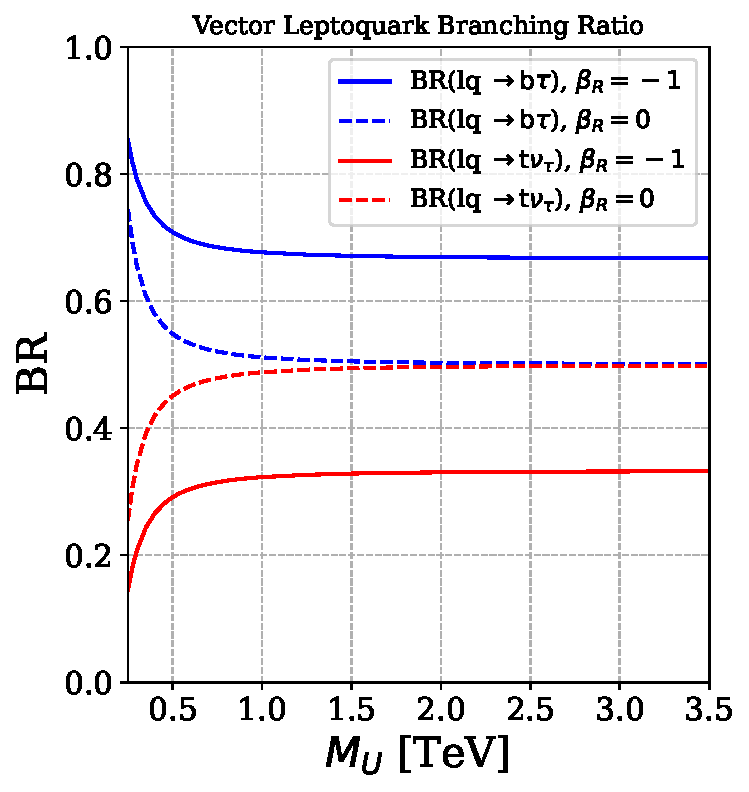
\includegraphics[width=.8\linewidth]{images/VLQ_BranchingRatio.pdf}
    \end{subfigure}
    \begin{subfigure}[b]{.94\linewidth}
    % 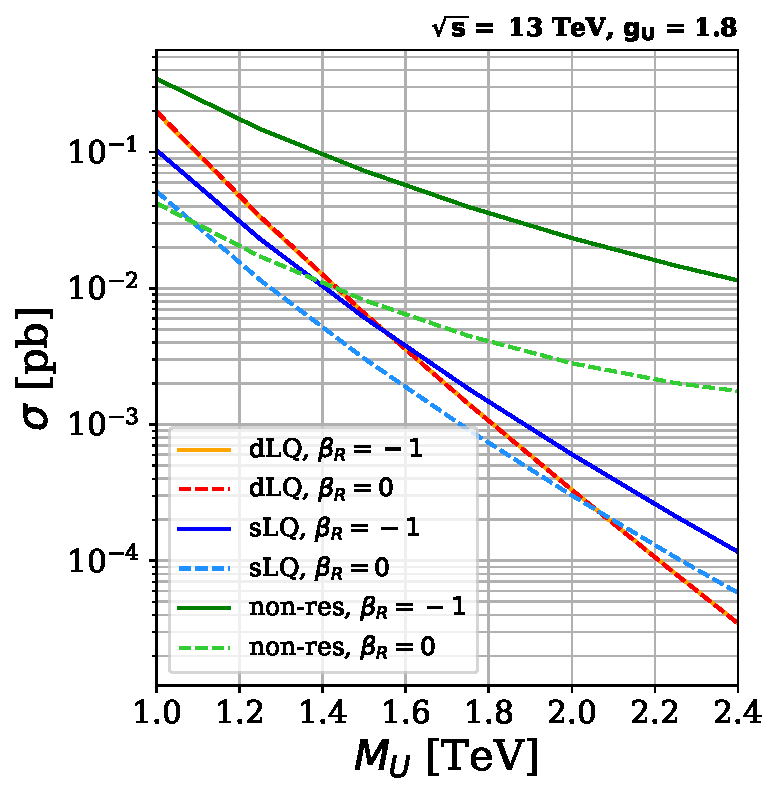
\includegraphics[width=.8\linewidth]{images/prod_cross_section_13TeV.pdf}
    \end{subfigure}
    \caption{Top: The $\lq\to\textrm{b}\tau$ and $\lq\to\textrm{t}\nu$ branching ratios for $\beta_{R} = 0$ (solid lines) and $\beta_{R} = -1$ (dashed lines). Bottom: Signal cross-section as a function of the $\lq$ mass, for $\sqrt{ s}=13 \tev$, with $g_U=1.8$. We show single, pair, and non-resonant production, for $\beta_R=-1,\,0$ in solid and dashed lines, respectively.}
\label{fig:branching_ratios}
\end{figure}

To further understand the role of $\beta_R$ at colliders, Figure~\ref{fig:branching_ratios} (bottom) shows the cross-section for single-$\lq$ (s$\lq$), double-$\lq$ (d$\lq$), and non-resonant (non-res) production, as a function of mass and for a fixed coupling $g_{U} = 1.8$, assuming $\mathrm{p}\,\mathrm{p}$ collisions at $\sqrt{s} = 13$ $\tev$. We note that this benchmark scenario with $g_{U}=1.8$ results in a $\lq\to\textrm{b}\tau$ decay width that is $<$5\% of the $\lq$ mass, for mass values from 250 $\gev$ to 2.5 $\tev$. In the Figure, we observe that, since d$\lq$ production is mainly mediated by events from quantum chromodynamic processes, the choice of $\beta_R$ does not affect the cross-section. However, for  s$\lq$ production, a non-zero value for $\beta_R$ increases the cross-section by about a factor of 2 and by almost one order of magnitude in the case of non-res production. These results shown in Figure~\ref{fig:branching_ratios} are easily understood by considering the diagrams shown in Figure~\ref{fig:feynmp-prod-channels}. The $\lq$ mass value where the s$\lq$ production cross-section exceeds the d$\lq$ cross-section depends on the choice of $g_U$. 
 
We also note that to solve the $R_{D^{(*)}}$ anomaly, the authors of~\cite{Cornella:2021sby} point out that the wilson coefficient $C_U\equiv g^2_U\,v^2_{SM}/(4\,M^2_U)$ is constrained to a specific range of values, and this range depends on the value of the $\beta_{R}$ parameter. Therefore, the allowed values of the coupling $g_{U}$ depend on $M_{U}$ and $\beta_{R}$, and thus our studies are performed in this multi-dimensional phase space.


As noted in section~\ref{sec:intro}, we study the role of a $\zb'$ boson in $\mathrm{p}\,\mathrm{p}\to\tau\tau$ production. The presence of a $\zb'$ boson in $\lq$ models has been justified in various papers, for example, in~\cite{Baker:2019sli}. The argument is that minimal extensions of the SM which include a massive gauge $U_1$ LQ, uses the gauge group $SU(4)\times SU(3)^{\prime}\times SU(2)_L \times U(1)_{T_R^3}$. Such an extension implies the presence of an additional massive boson, $\zb^{\prime}$, and a color-octet vector, $G'$, arising from the spontaneous symmetry breaking into the SM \marginpar{Naively, the LQs are associated to the breaking of $SU(4)\to SU(3)_{[4]}\times U(1)_{B-L}$, the $G'$ arises from $SU(3)_{[4]}\times SU(3)'\to SU(3)_c$, and the $Z'$ comes from the breaking of $U(1)_{B-L}\times U(1)_{T_R^3}\to U(1)_Y$. Notice that the specific pattern of breaking, and the relations between the masses and couplings, are connected to the specific scalar potential used.}.  The $\zb'$ in particular can play an important role in the projected $\lq$ discovery reach, as it can participate in $\mathrm{p}\,\mathrm{p}\to\tau\tau$ production by s-channel exchange, both resonantly and as a virtual mediator. To study the effect of a $\zb'$ on the $\mathrm{p}\,\mathrm{p}\to\tau\tau$ production cross-sections and kinematics, we extend our benchmark Lagrangian in Eq.~(\ref{eq:BasicLagrangian}) with further non-renormalizable terms involving the $\zb'$. Accordingly, we assume the $\zb'$ only couples to third-generation fermions. Our simplified model is thus extended by:
\begin{eqnarray}
    \label{eq:BasicLagrangianZp}
        \mathcal{L}_{Z^{\prime}}&= & -\frac{1}{4} Z_{\mu \nu}^{\prime} Z^{\prime \mu \nu}+\frac{1}{2} M_{Z^{\prime}}^2 Z_\mu^{\prime} Z^{\prime \mu} \nonumber \\
        && + \frac{g_{Z^{\prime}}}{2 \sqrt{6}} Z^{\prime \mu} (\zeta_q \bar{Q}_3 \gamma_\mu Q_3 \nonumber +\zeta_t \bar{t}_R \gamma_\mu t_R \\
        &&  +\zeta_b \bar{b}_R \gamma_\mu b_R-3 \zeta_{\ell} \bar{L}_3 \gamma_\mu L_3-3 \zeta_\tau \bar{\tau}_R \gamma_\mu \tau_R)
\end{eqnarray}
where the constants $M_{\zb^{\prime}}$, $g_{Z^{\prime}}$, $\zeta_q $, $\zeta_t $, $\zeta_b$, $\zeta_{\ell}$, $\zeta_\tau$, are model dependent.

We study two extreme cases for the $\zb'$ mass, following~\cite{GINO_PhysRevD.102.115015}, namely $M_{\zb'} = \sqrt{\tfrac{1}{2}}M_U<M_U$ and $M_{\zb'} = \sqrt{\tfrac{3}{2}}M_U>M_U$. We also assume the $\lq$ and $\zb'$ are uniquely coupled to left-handed currents, i.e. $\zeta_q=\zeta_\ell= 1$ and $\zeta_t=\zeta_b=\zeta_\tau=0$. With these definitions, Figure~\ref{fig:xsinterference} shows the effect of the $\zb'$ on the $\tau\tau$ production cross-section, considering $g_U = 1$, $\beta_R=0$, and different $g_{\zb^{\prime}}$ couplings. On the top panel, the cross-sections corresponding to the cases where $M_{\zb'} = \sqrt{\tfrac{1}{2}}M_U$ are shown. As expected, the $\tau\tau$ production cross-section for the inclusive case (i.e., $g_{\zb'} \neq 0$) is larger than that for the $\lq$-only non-res process ($g_{\zb'} = 0$, depicted in blue). This effect increases with $g_{\zb'}$ and, within the evaluated values, can exceed the $\lq$-only cross-section by up to two orders of magnitude. In contrast, a more intricate behaviour can be seen in the bottom panel of Figure~\ref{fig:xsinterference}, which corresponds to $M_{\zb'} = \sqrt{\tfrac{3}{2}}M_U$. Here, for low values of $M_U$, a similar increase in the cross-section is observed. However, for higher values of $M_U$, the inclusive $\mathrm{p}\,\mathrm{p}\to\tau\tau$ cross-section is smaller than the $\lq$-only $\tau\tau$ cross-section. This behaviour suggests the presence of a dominant destructive interference at high masses, leaving its imprint on the results.
\begin{figure}[]
\centering
    \begin{subfigure}[b]{.94\linewidth}
    % 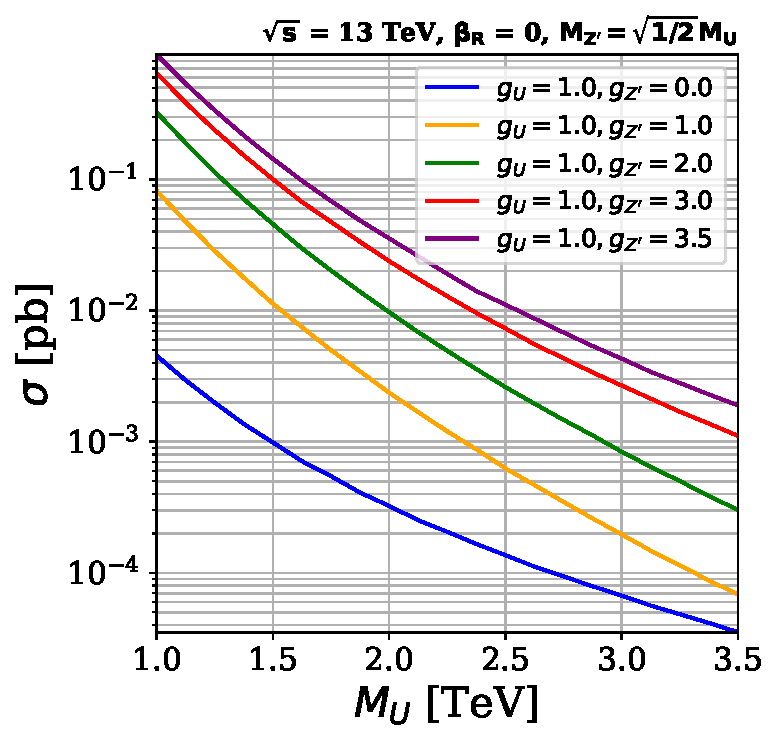
\includegraphics[width=.8\linewidth]{images/XS_gu_gzp_lower_limit_woRHC.pdf}
    \end{subfigure}
    \begin{subfigure}[b]{.94\linewidth}
    % 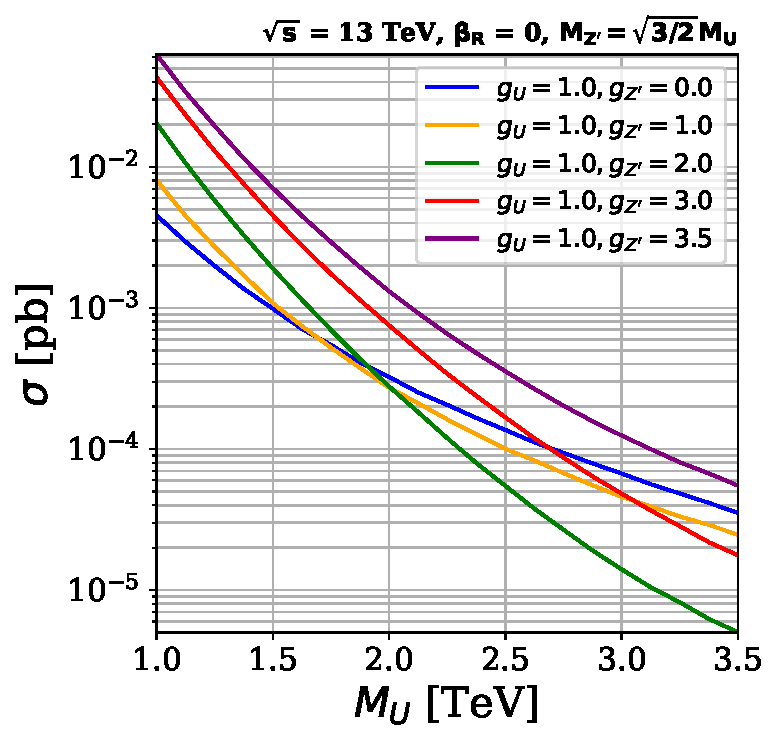
\includegraphics[width=.8\linewidth]{images/XS_gu_gzp_upper_limit_woRHC.pdf}
    \end{subfigure}
    \caption{$\tau \tau$ cross-section as a function of the $\lq$ mass for different values of $g_U$ and $g_{\zb^{\prime}}$. The estimates are performed at $\sqrt s=13 \tev$, $\beta_R=0$,  $M_{\zb^{\prime}} = \sqrt{1/2} M_{U}$ (top), and $M_{\zb^{\prime}} = \sqrt{3/2} M_{U}$ (bottom).}
\label{fig:xsinterference}
\end{figure}

\begin{figure}[]
\centering
    \begin{subfigure}[b]{.94\linewidth}
    % 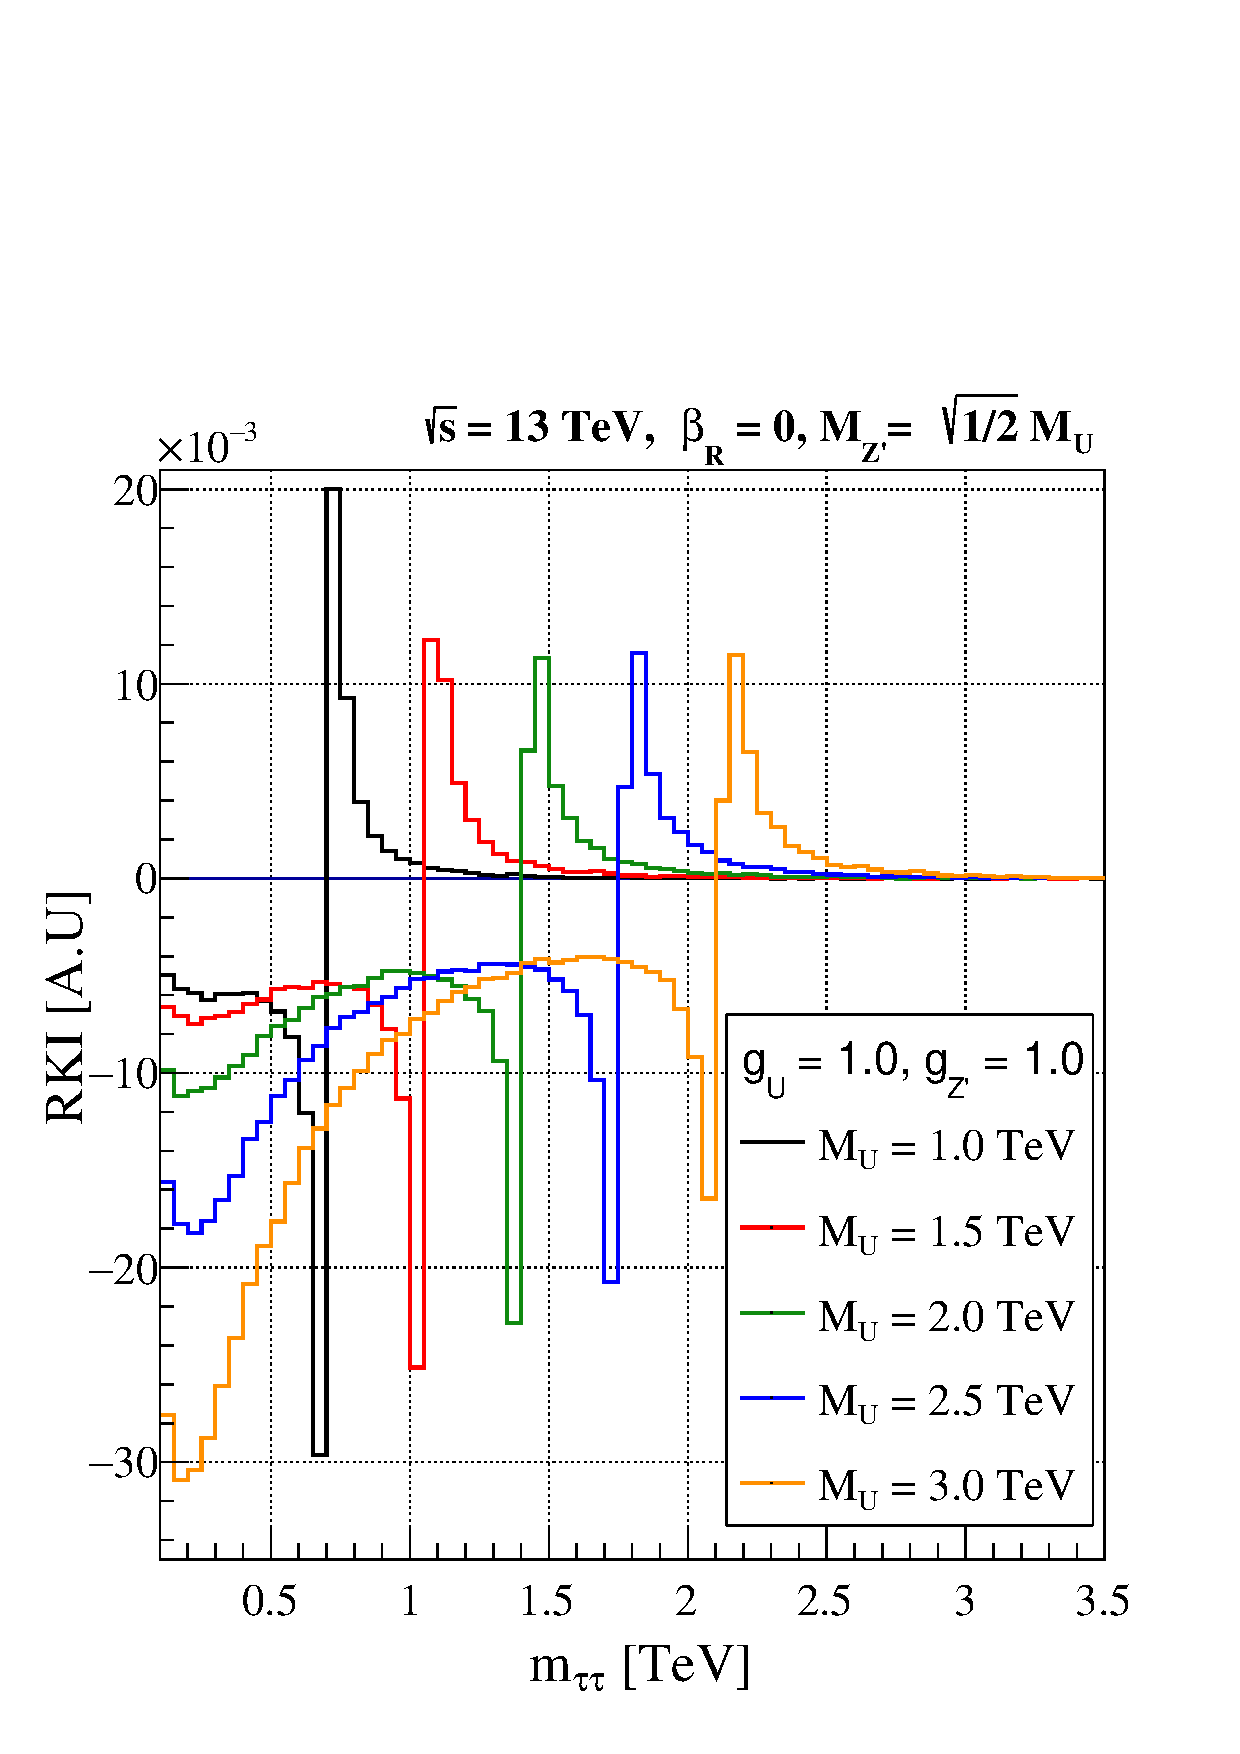
\includegraphics[height=6cm, width=6.0cm]{images/Kinematic_Interference_gu_1.0_gzp_1.0_zp_lower_limit_woRHC.pdf}
    \end{subfigure}
    \begin{subfigure}[b]{.94\linewidth}
    % 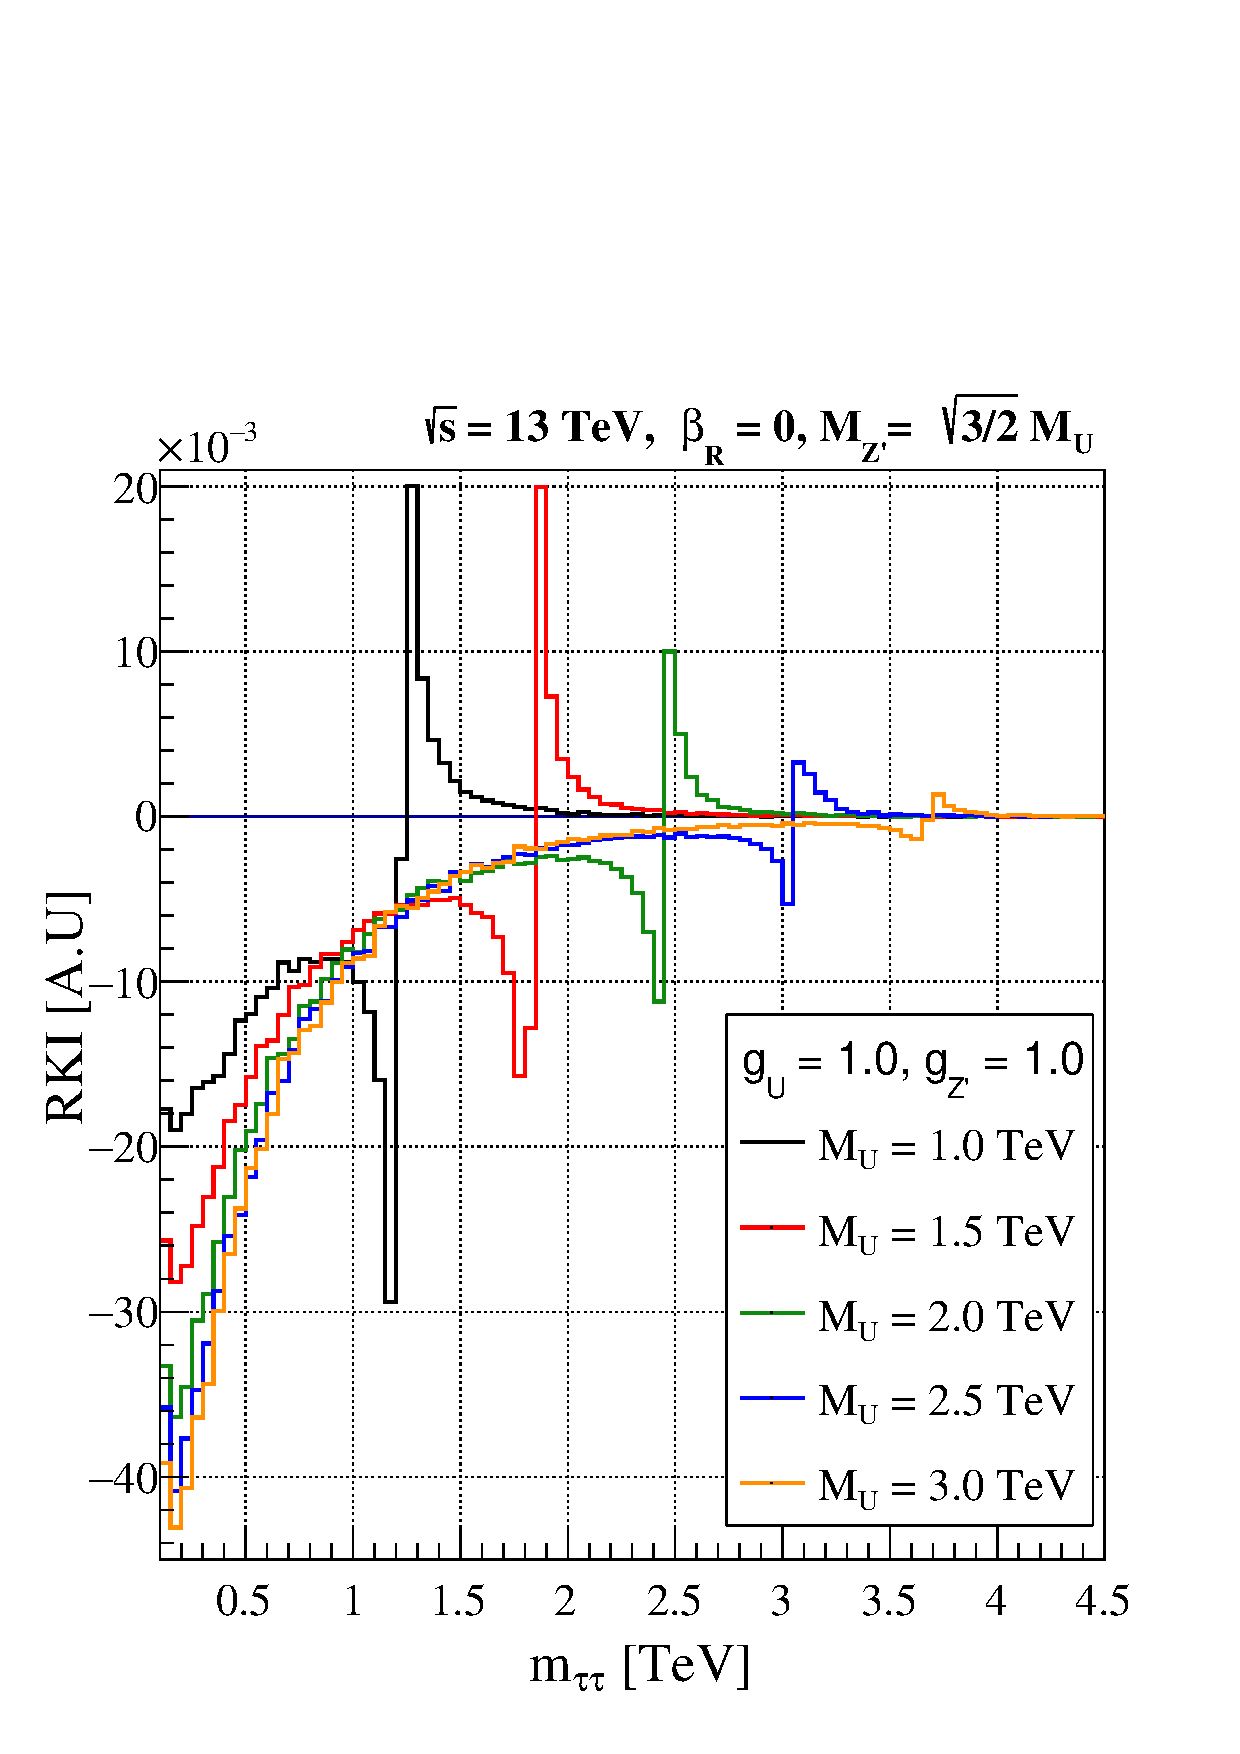
\includegraphics[height=6cm, width=6cm]{images/Kinematic_Interference_gu_1.0_gzp_1.0_zp_upper_limit_woRHC.pdf}
    \end{subfigure}
    \caption{The relative kinematic interference (RKI), as a function of the reconstructed mass of two taus, for different $\lq$ masses. The studies are performed assuming $\sqrt s=13 \tev$, $\beta_R=0$, $g_U = 1.0$, $g_{\zb^{\prime}} =1.0$, $M_{\zb^{\prime}} = \sqrt{1/2} M_{U}$ (top), and $M_{\zb^{\prime}} = \sqrt{3/2} M_{U}$ (bottom).
    }    
\label{fig:interference}
\end{figure}
In order to further illustrate the effect, Figure~\ref{fig:interference} shows the relative kinematic interference ($\mathrm{RKI}$) as a function of the reconstructed invariant mass $m_{\tau\tau}$, for $g_{\zb^{\prime}} = 1$ and varying values of $M_U$. The RKI parameter is defined as
\begin{equation}
    \mathrm{RKI}(m_{\tau\tau})=\frac{1}{\sigma_{\lq+\zb'}}\left[\frac{d\sigma_{\lq+\zb'}}{dm_{\tau\tau}}-\left(\frac{d\sigma_{\lq}}{dm_{\tau\tau}}+\frac{d\sigma_{\zb'}}{dm_{\tau\tau}}\right)\right],
\end{equation}
where $\sigma_{X}$ is the production cross-section arising due to contributions from $X$ particles. For example, $\sigma_{\lq+\zb'}$ represents the inclusive cross-section where both virtual $\lq$ and s-channel $\zb'$ exchange contribute. For both cases, we can observe the presence of deep valleys in the RKI curves when $m_{\tau\tau}\to0$, indicating destructive interference between the $\lq$ and the $\zb'$ contributions. This interference generates a suppression of the differential cross-section for lower values of $m_{\tau\tau}$ and, therefore, in the integrated cross-section. 
 
The observed interference effects are consistent with detailed studies on resonant and non-res $\mathrm{p}\,\mathrm{p}\to\tq \bar{\tq}$ production, performed in reference~\cite{Djouadi:2019cbm}.